\section{Demarche Expérimentale}

\begin{figure}[h]
    \centering
    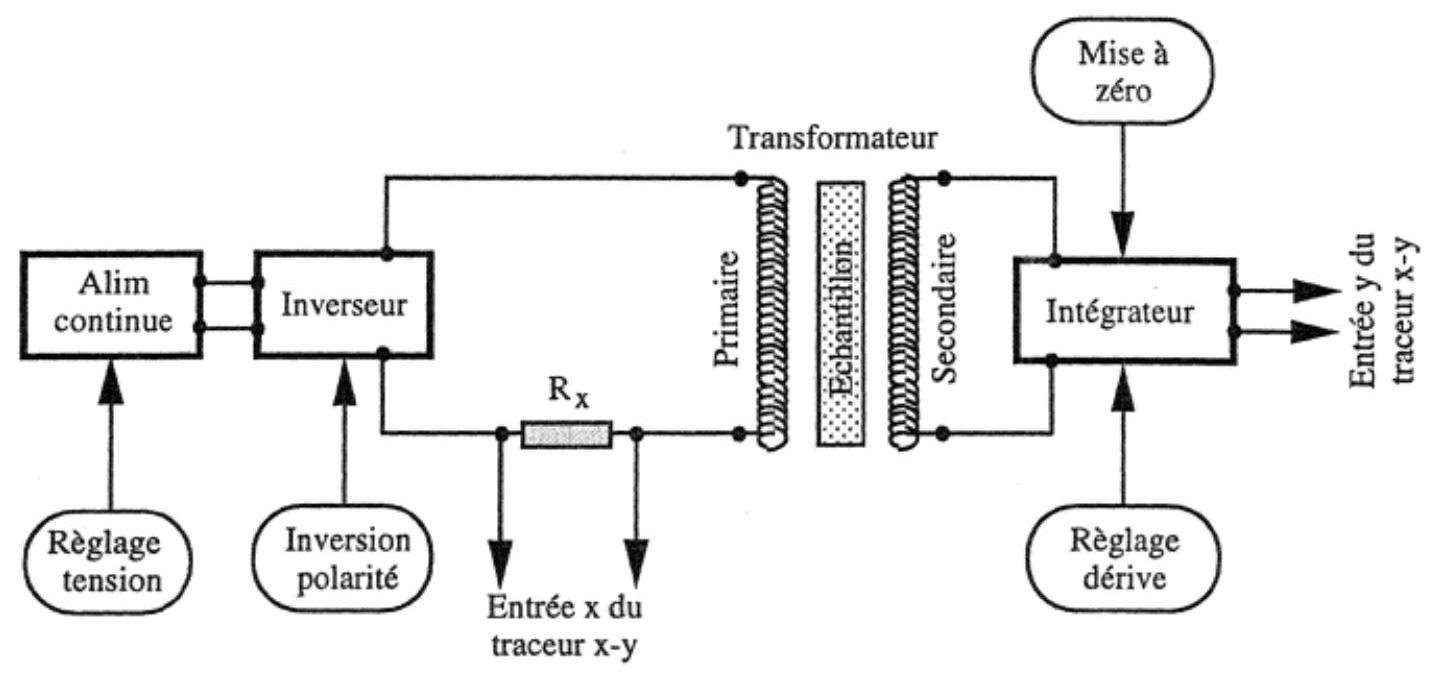
\includegraphics[width=0.8\linewidth]{figures/montage.png}
    \caption{Schéma du montage expérimental \cite{notice}}
    \label{fig:montage}
\end{figure}

Afin de déterminer la perméabilité magnétique de différents matériaux, le montage à la \autoref{fig:montage} est utilisé. Deux transformateurs sont utilisés.

\begin{enumerate}
    \item Un transformateur PHYWE, composé d'un noyau en acier en forme de "U" sur lequel il est possible de mettre une bobine primaire et une bobine secondaire, qu'il est possible de changer afin de règler la sensibilité du transformateur. Pour cette expérience une bobine primaire de 600 spires et une bobine secondaire de 1200 spires ont été utilisés. Le transformateur peut être fermé avec les échantillons à tester ou avec un bloc spécial fourni.
    \item Un transformateur cylindrique, composé d'une bobine primaire de 405 spires et une bobine secondaire de 4920 spires. Les échantillons cylindriques sont inserés à l'intérieur du cylindre.
\end{enumerate}

Pour s'assurer qu'un échantillon ne soit pas magnétisé avant les mesures, une mise à zero est nécessaire en mettant l'échantillon dans le transformateur puis en faisant varier la tension pour que l'induction magnétique soit nulle. Il est également nécessaire de s'assurer que l'intégrateur ne dérive pas entre chaque mesure. Pour chaque échantillon, la tension est variée sur un cycle \(0 \rightarrow V_+ \rightarrow V_- \rightarrow 0 \rightarrow V_+\). Les valeurs \((V_x, V_y)\) sont relevées automatiquement par le ploteur X-Y, où \(V_x\) est la tension d'entrée mesurée aux bornes d'une resistance \((1.00 \pm 0.01)\) \si{\ohm} à l'entrée du transformateur et \(V_y\) est l'intégrale de la tension de sortie du transformateur.

À l'aide des \autoref{eq:calibr_H} et \autoref{eq:calibr_B}, il est possible d'obtenir les valeur du champ magnétique \(H_m\) et \(H_s\) pour les cycles.
